\documentclass[../main.tex]{subfiles}

\begin{document}
    Para obtener la altura $D$, integraremos la ecuación hidrostática, obteniendo así la siguiente expresión
    \begin{equation}
        P_2 - P_1 = -\rho g D
    \end{equation}
Con $g = 9.78 \text{m/s}^{2}$ la aceleración de gravedad, y $\rho = 997 \text{ Kg/m}^3$ la densidad del agua líquida.

Luego, tenemos que 
\begin{equation}
    D = \frac{e_1-e_2}{\rho g} \label{D}
\end{equation}
donde hemos remplazado $P$ por $e$, ya que el gas al interior del pato es solo vapor de agua.\\

Notemos que estamos considerando $e_1$ la presión del vapor en la base del pato, y $e_2$ el vapor en la parte superior del pato.\\

Como tenemos la temperatura (20 $^\circ$C) y humedad relativa del ambiente (50$\%$), podemos obtener la temperatura punto de bulbo húmedo del ambiente, usando el gráfico Skew T (asumiendo una presión de unos 1000 hPa). Luego, como el vapor de está en contacto con agua líquida, sabemos que su presión será igual a la presión de vapor saturada, por lo que usando la ecuación de Clasius-Clapeyron podemos obtener $e_1$ y $e_2$.\\

\begin{minipage}{\linewidth}
    \centering
        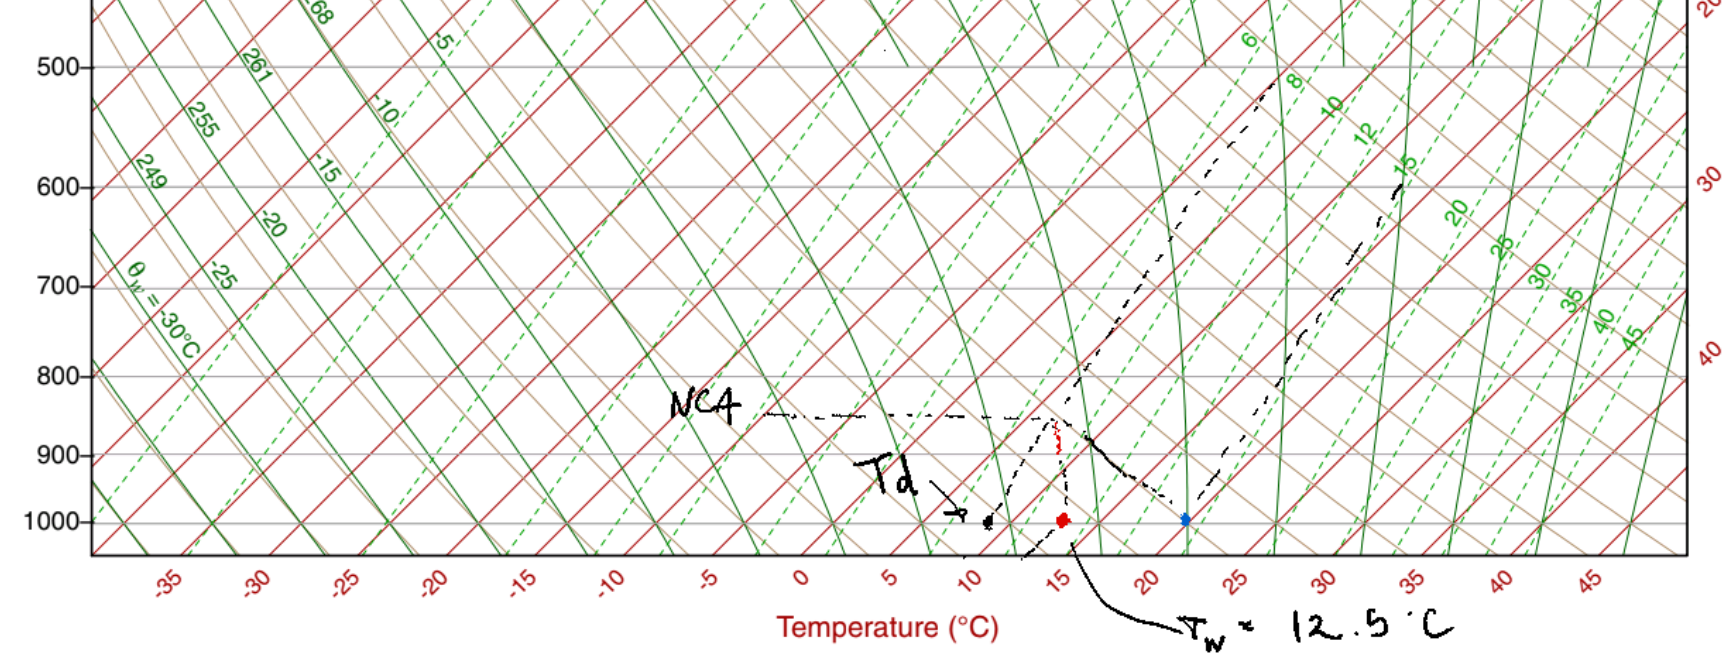
\includegraphics[width=0.95\textwidth]{img/skewT}
        \captionof{figure}{Gráfico SkewT - LogP. El punto azul muestra la temperatura medida. El punto negro muestra la temperatura punto de rocío, y finalmente el punto rojo muestra la temperatura de bulbo húmedo.}
        \label{fig:skewT}
\end{minipage}\\

Como se observa en la \autoref{fig:skewT}, se reconoce del punto azul una razón de mezcla saturada de $w_\text{sat} \simeq 14$ g/Kg. Luego, como la humedad relativa es del $50\%$, la temperatura punto de rocío se encuentra (al mismo nivel de presión) donde la razón de mezcla saturada es de 7 g/Kg. \\

Consideramos que la parcela del punto azul asciende adiabáticamente y también que una parcela del punto negro asciende a razón de mezcla constante. Identificamos el punto donde ambas trayectorias se intersectan para luego descender por un camino adiabático húmedo hasta alcanzar el nivel de presión inicial. De este modo vemos que la temperatura de bulbo húmedo es $T_w \simeq 12.5\,^{\circ}\text{C}$.\\

Ahora usaremos la ecuación de Clasius-Clapeyron
\begin{equation}
   e_\text{sat}(T) = 6.11 \cdot \exp \left(   5.42\cdot 10^3 \left( \frac{1}{273} - \frac{1}{T} \right) \right)
\end{equation}
con $T$ la temperatura en Kelvin. De esto obtenemos que 
 \begin{equation}
     e_1 = e_\text{sat}(T = 20^{\circ}\text{C}) \simeq 23.7 \text{ hPa,} \label{e1}
 \end{equation}
\begin{equation}
    e_2 = e_\text{sat}(T = 12.5^{\circ}C) \simeq 14.6 \text{ hPa.} \label{e2}
\end{equation}

Finalmente, evaluando \eqref{e1}, \eqref{e2}, y el resto de los valores numéricos mencionados anteriormente, en la ecuación \eqref{D}, obtenemos que $D$ es aproximadamente 9.35 centímetros.\\

Respecto a porque es mejor usar líquidos más volátiles, creo que que es principalmente a que la curva de Clasius-Clapeyron para los vapores de dichos gases queda más ``empinada'' o está desplazada hacia la izquierda, respecto a la curva para el vapor de agua. Mostramos en la \autoref{fig:eT} por ejemplo, como una curva más empinada/desplazada (curva roja) respecto a una pequeña variación en la temperatura (en el rango de temperatura ambiente), presenta una alta variación en su presión de vapor. \\

\begin{minipage}{\linewidth}
    \centering
    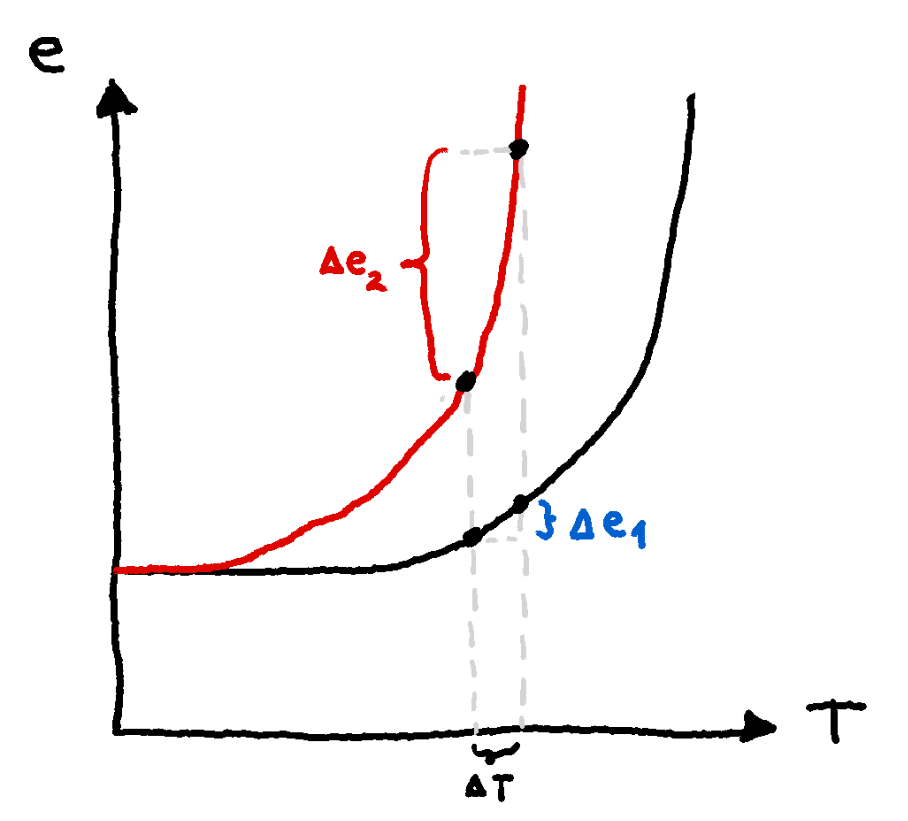
\includegraphics[width=0.45\textwidth]{img/eT}
    \captionof{figure}{La curva satura representa la curva $e_\text{sat}$ para el vapor de agua, mientras que la curva roja, para el vapor de un líquido más volátil. Se aprecia que $\Delta e_2 > \Delta e_1.$}
    \label{fig:eT}
\end{minipage}



\end{document}
